\documentclass[11pt]{article}
\usepackage[margin=1in]{geometry}
\usepackage{amsmath,amssymb,amsthm}
\usepackage{graphicx}
\usepackage[hidelinks]{hyperref}

\newtheorem{theorem}{Theorem}
\newtheorem{lemma}{Lemma}

\title{Endpoint failure when cotype is not attained}
\author{Run fa\_banach\_001, agent\_lane\_15}
\date{June 28, 2026}

\begin{document}
\maketitle

\begin{abstract}
Aron et al. prove an optimal Hardy--Littlewood theorem for range spaces that
attain their cotype, and an \(\varepsilon\)-shifted theorem for finite-cotype
spaces when cotype attainment is not known.  We show that the epsilon loss is
necessary in general.  There is an explicit infinite-dimensional Banach space
\(Y\) with \(\cot Y=2\), not of cotype \(2\), and a bounded linear operator
\(A:\ell_4\to Y\) for which \((\|Ae_j\|)_j\notin \ell_4\).
\end{abstract}

\section{Source context}

The source paper is arXiv:1602.00178v4, ``Optimal exponents for
Hardy--Littlewood inequalities for \(m\)-linear operators''
\cite{aron1602}.  Its main vector-valued result assumes that the target
Banach space \(Y\) attains its cotype.

\begin{center}
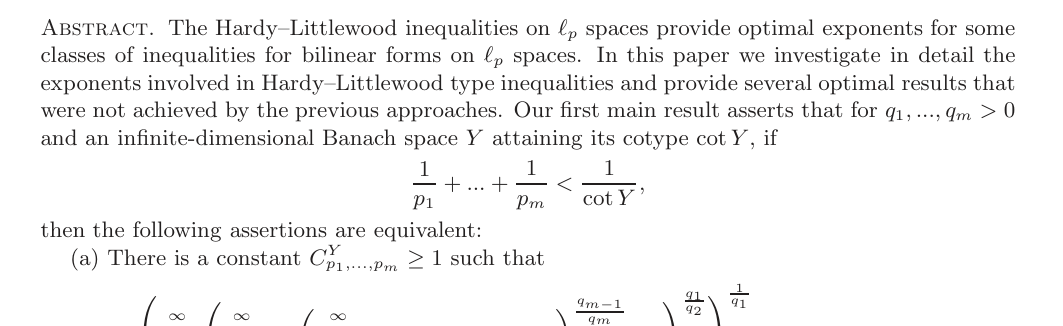
\includegraphics[width=0.9\linewidth]{figures/main_theorem_crop.png}
\end{center}

Later, the paper treats the case where one does not know if \(Y\) attains the
infimum of its cotypes, but the conclusion is weakened by replacing each
endpoint exponent \(q_j\) by \(q_j+\varepsilon\).

\begin{center}
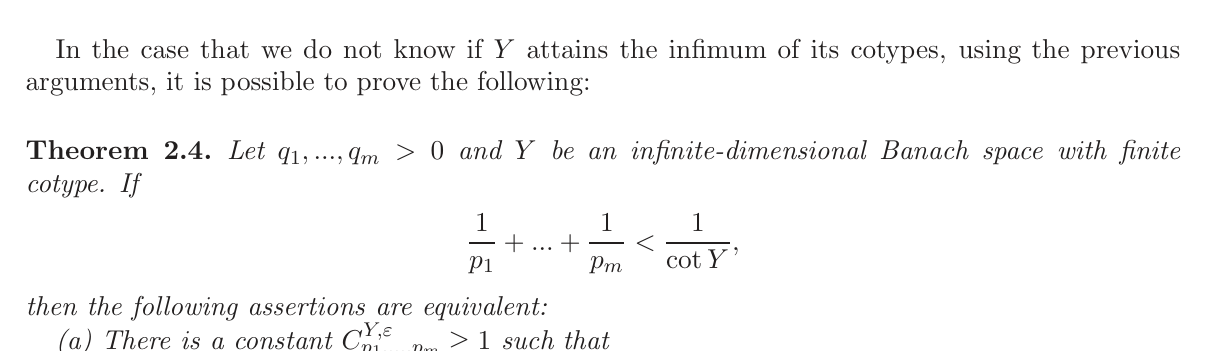
\includegraphics[width=0.9\linewidth]{figures/nonattained_cotype_crop.png}
\end{center}

The construction below shows that this endpoint loss is not merely an artifact
of the proof.

\section{Idea of the proof}

If a Banach space has cotype \(s\) for every \(s>2\), but not cotype \(2\),
then \(\cot Y=2\) is not attained.  We build such a space from finite blocks
\(\ell_{2+1/n}^{N_n}\), choosing the dimensions \(N_n\) so large that the
cotype \(2\) constants of the blocks diverge.  The same oversized blocks let
us construct a bounded block-diagonal operator \(A:\ell_4\to Y\).  Each block
is scaled just enough to keep the operator bounded, but not enough to make the
endpoint coefficient sequence \((\|Ae_j\|)\) belong to \(\ell_4\).

\section{The counterexample}

\begin{theorem}
\label{thm:endpoint-failure}
There is an infinite-dimensional Banach space \(Y\) with finite cotype and
\(\cot Y=2\), but not of cotype \(2\), such that the endpoint linear
Hardy--Littlewood inequality predicted by the epsilon-free version of Theorem
2.4 in \cite{aron1602} fails.  More precisely, there is a bounded operator
\[
A:\ell_4\longrightarrow Y
\]
such that
\[
\sum_{j=1}^{\infty}\|A e_j\|_Y^4=\infty.
\]
\end{theorem}

\begin{proof}
For \(n\ge1\), put
\[
r_n=2+\frac1n,\qquad N_n=n^{4n+2},\qquad
E_n=\ell_{r_n}^{N_n},
\]
and define
\[
Y=\left(\bigoplus_{n=1}^{\infty}E_n\right)_2.
\]

First we record the cotype of \(Y\).  The space \(Y\) has cotype \(s\) for
every \(s>2\).  Indeed, for all sufficiently large \(n\) one has \(r_n\le s\),
and the standard cotype theorem for \(L_p\)-spaces gives uniformly bounded
cotype \(s\) constants for the blocks \(\ell_{r_n}^{N_n}\) with \(r_n\in[2,s]\);
the finitely many remaining blocks are harmless.  An \(\ell_2\)-sum of spaces
with uniformly bounded cotype \(s\) again has cotype \(s\).  Hence
\(\cot Y\le2\), and since cotype exponents are always at least \(2\), we have
\(\cot Y=2\).

But \(Y\) is not of cotype \(2\).  Each block \(E_n\) is 1-complemented in
\(Y\).  Applying a cotype \(2\) inequality to the unit vector basis of
\(\ell_{r_n}^{N_n}\) would force its cotype \(2\) constant to be at least
\[
\frac{N_n^{1/2}}{N_n^{1/r_n}}
=N_n^{1/2-1/r_n}
=\left(n^{4n+2}\right)^{1/(4n+2)}
=n.
\]
These lower bounds are unbounded, so \(Y\) cannot have cotype \(2\).

Now split the canonical basis of \(\ell_4\) into consecutive blocks of
cardinalities \(N_n\), and write \(x^{(n)}\in\ell_4^{N_n}\) for the \(n\)-th
block of \(x\in\ell_4\).  Define \(A:\ell_4\to Y\) blockwise by
\[
(Ax)_n
=
\frac1n\,N_n^{-(1/r_n-1/4)}\,x^{(n)}
\quad\in \ell_{r_n}^{N_n},
\]
where \(x^{(n)}\) is identified with the same coordinate vector in
\(\ell_{r_n}^{N_n}\).  Since the identity
\(\ell_4^{N_n}\to\ell_{r_n}^{N_n}\) has norm
\(N_n^{1/r_n-1/4}\), each block operator has norm at most \(1/n\).  Therefore
\[
\|Ax\|_Y^2
\le
\sum_{n=1}^{\infty}\frac1{n^2}\|x^{(n)}\|_4^2
\le
\left(\sum_{n=1}^{\infty}\frac1{n^4}\right)^{1/2}
\left(\sum_{n=1}^{\infty}\|x^{(n)}\|_4^4\right)^{1/2},
\]
so \(A\) is bounded from \(\ell_4\) to \(Y\).

For a basis vector \(e_j\) in the \(n\)-th block,
\[
\|Ae_j\|_Y
=
\frac1n\,N_n^{-(1/r_n-1/4)}.
\]
Thus
\[
\sum_j \|Ae_j\|_Y^4
=
\sum_{n=1}^{\infty}
N_n\frac1{n^4}N_n^{-4(1/r_n-1/4)}
=
\sum_{n=1}^{\infty}
\frac1{n^4}N_n^{1-4(1/r_n-1/4)}.
\]
Since
\[
1-4\left(\frac1{r_n}-\frac14\right)
=2-\frac4{2+1/n}
=\frac{2}{2n+1},
\]
we get
\[
\frac1{n^4}N_n^{1-4(1/r_n-1/4)}
=
\frac1{n^4}\left(n^{4n+2}\right)^{2/(2n+1)}
=1.
\]
Consequently \(\sum_j\|Ae_j\|_Y^4=\infty\).

For \(m=1\), \(p=4\), and \(\cot Y=2\), the endpoint exponent in the source
notation is
\[
\lambda_{1,2}^4=\frac{2}{1-\frac{2}{4}}=4.
\]
So the endpoint, epsilon-free version of Theorem 2.4 would assert precisely
that \((\|Ae_j\|)_j\in\ell_4\) for every bounded \(A:\ell_4\to Y\), which the
operator above disproves.
\end{proof}

\section{Verification notes}

The included script \texttt{code/nonattained\_cotype\_endpoint\_check.py}
checks the exponent identities
\[
N_n^{1/2-1/r_n}=n,\qquad
n^{-4}N_n^{1-4(1/r_n-1/4)}=1.
\]
These identities are the two quantitative cores of the proof: the first shows
non-attainment of cotype \(2\), and the second shows divergence of the endpoint
\(\ell_4\) coefficient sum.

\section{Novelty and limitations}

Local run indexes were searched for arXiv:1602.00178, Hardy--Littlewood,
optimal exponents, multilinear forms, cotype, and non-attained cotype.  No
exact prior packet was found.  Bounded web searches on June 28, 2026 for the
source arXiv id, Hardy--Littlewood cotype endpoint, and non-attained-cotype
epsilon language found no separate known answer beyond the source arXiv
record.

The packet does not contradict Theorem 2.4 of \cite{aron1602}, because that
theorem includes an \(\varepsilon\)-shift in every exponent.  The result shows
that this shift cannot be removed for arbitrary finite-cotype target spaces.
The counterexample already occurs in the linear case \(m=1\); it therefore
also blocks any multilinear theorem that would include the linear endpoint as
a special case.

\section{Human-review recommendation}

The key review point is the standard cotype calculation for
\(\ell_2\)-sums of finite-dimensional \(\ell_r\) blocks.  Once that is
accepted, the endpoint failure is an explicit block-diagonal operator
calculation.

\begin{thebibliography}{9}
\bibitem{aron1602}
R. M. Aron, D. Nunez-Alarcon, D. M. Pellegrino, and
D. M. Serrano-Rodriguez,
\emph{Optimal exponents for Hardy--Littlewood inequalities for \(m\)-linear
operators},
arXiv:1602.00178v4, 2016.
\url{https://arxiv.org/abs/1602.00178}.
\end{thebibliography}

\end{document}
